%-------------------------------------------------------------------------------
% Fichero:	Pinguino.tex
% Documento:	Un quick hacking para Bricolabs
% Autor:	Sergio Alvariño (salvari)
% Fecha:        Sun Jun  2 00:49:00 2013
% Descripción:	Un howto del Pinguino
% Versión:      0.00
% Historial:    0.00 (Sun Jun  2 00:49:00 2013): Primera versión
% TODO: Añadir una sección con las consideraciones necesarias para celebrar un QH
%       Añadir una sección comparativa de micros arduino - pinguino
%-------------------------------------------------------------------------------

\documentclass[12pt,a4paper,twoside,DIV=15]{scrartcl}
\usepackage{bookman}

% Esto es para poder escribir acentos directamente:
\usepackage[utf8]{inputenc}
% Esto es para que el LaTeX sepa que el texto está en español:
\usepackage[spanish]{babel}

\usepackage[pdftex]{graphicx}
\DeclareGraphicsExtensions{.pdf,.png,.jpg} %solo para PDFLaTeX
\graphicspath{{figures/}{graphics/}}
% \loadgraphics[<bb>]{miLogoVodafone.ps}

\usepackage{hyperref}

% Header and footers
% \usepackage[automark]{scrpage2}
\usepackage{scrpage2}
% \ihead[scrplain-inside]{scrheadings-inside}
% \chead[\headmark]{\headmark}
\chead[Bricolabs Quick Hacking: Pingüino ]{Bricolabs Quick Hacking Pingüino}
\ohead[]{

\includegraphics [scale=.09]{pinguino.png}

}
% \ifoot[scrplain-inside]{scrheadings-inside}
\cfoot[Bricolabs Quick Hacking]{Bricolabs Quick Hacking}
\ofoot[\pagemark]{\pagemark}
%\automark

\pagestyle{scrheadings}


%\usepackage{array}		%
%\usepackage{tabularx}		% Junto con Array, para hacer tablas


%--------------------------------------------------------------------------
% Atajos.

%--------------------------------------------------------------------------
% Comandos de fuente
\newcommand{\ext}[1]{\emph{#1}}	% Para todo lo que esté en
                                % extranjero

%----------------------------------------
% Nuevos entornos
\newenvironment{nota}%
{% Comienzo -----------------------------
\begin{table}[h]\centering
\begin{tabular}{ |p{12cm}|}%
\hline%
\textbf{Nota:}%
}%
{% Final --------------------------------
\hline%
\end{tabular}%
\end{table}
}


%--------------------------------------------------------------------------
% Página de título
% \titlehead{Titlehead }
% \subject{Subject }
% \title{Title }
% \subtitle{Subtitle }
% \author{Author }
% \date{Date }
% \publishers{Publisher }
% \and
% \thanks{Footnote }


\title{Conociendo al Pingüino}
\subtitle{Propuesta de ``Quick Hacking''}
\author{Bricolabs\\
  \small salvari@gmail.com\\
}
\date{\small Junio 2013}


\begin{document}
\maketitle

\abstract{Propuesta de Quick Hacking para Bricolabs: Montaje de un
  Pingüino de 8 bits e instalación del IDE en Ubuntu Linux.  

  Este trabajo no está completo, se harán correcciones y añadidos}

\tableofcontents
\section{Introducción}
\label{sec:introduccion}

Pingüino es un proyecto OSOH, que consisten en una combinación de IDE
y compiladores basados en software libre y diseños hardware basados en
microcontroladores PIC del fabricante Microchip (de 8 y 32 bits). El
objetivo del proyecto es desarrollar un plataforma similar a Arduino y
compatible con el mismo.

\begin{nota}
  Veo que ya te estás impacientando y no te vas a leer este rollo,
  pero te aconsejo que como mínimo te leas la sección
  \ref{sec:peculiar}. No sea que te pase como a mi y pierdas dos
  semanas.\\
\end{nota}

\subsection{¿Qué nos aporta Pingüino frente a Arduino?}
\label{sec:ventajas}

\begin{itemize}
\item A diferencia de Arduino, Pingüino es un proyecto de hardware y
  software abierto. Disponemos de multitud de diseños hardware
  liberados por la comunidad.
\item Pingüino incorpora un IDE programado en Python que soporta tanto
  microcontroladores de 8 bits como de 32 bits de Microchip.
\item Pingüino usa compiladores libres: SDCC (8 bits)  y GCC (32 bits)
\item Pingüino tiene como objetivo conseguir una compatibilidad total con Arduino
\item Los microcontroladores PIC incluyen, entre otras cosillas:
  \begin{itemize}
  \item Puerto USB
  \item Reloj y calendario de tiempo real
  \end{itemize}
\end{itemize}

Todo sería perfecto, sino fuese por la pegas que también las hay:

\subsection{Desventajas de Pingüino}
\label{sec:desventajas}

\begin{itemize}
\item Los microcontroladores PIC no incluyen las resistencias internas
  que incluye Arduino. Por lo tanto habrá que usar siempre
  resistencias externas en nuestros montajes.
\item La comunidad Pingüino es muchísimo más pequeña que la de Arduino.
  \begin{itemize}
  \item Eso implica que el desarrollo se lleva a cabo por voluntarios,
    en su tiempo libre. Los desarrollos software no son tan rápidos
    como en Arduino.
  \item Solo hay un par de fabricantes que hagan hardware Pingüino
    (pero siempre te puedes hacer tu el montaje)
  \end{itemize}
\item Para cargar un nuevo programa en el Pingüino es necesario pulsar
  un botón. No es automático como el Arduino.
\item No tenemos tantas librerias como para Arduino, no todas están
  portadas todavía.
\item Pingüino no es compatible con todos los shields Arduino, aunque
  cada vez hay más shields para Pingüino.
\item El entorno de desarrollo no incluye el terminal serie de
  depuración, será necesario usar terminales específicos\footnote{En
    Linux esto es fácil, hay multitud de terminales software}.
\end{itemize}

\section{¿Por qué un Pingüino?}
\label{sec:porque}

Bueno, hubo un tiempo en que no existía el Arduino y los PIC eran ``El
Microprocesador'', así que antes de entrar en Bricolabs y poner al dia
mis conocimientos del ``estado del arte'', todas mis búsquedas en
Google incluían los términos ``PIC microcontroller''. Con esas
busquedas coleccioné un montón de literatura basada en PIC.

Las herramientas de programación del fabricante (Microchip) son
todavía un poco deficientes para Linux. El fabricante ha portado su
entorno de desarrollo a Linux, pero el proceso de instalación es
super-intrusivo, y un poco chapucero en mi opinión.\footnote{El
  programa debe ejecutarse como root una vez instalado}. Buscando
alternativas encontré el proyecto Pingüino.

El proyecto es completamente abierto, en el aspecto hardware y
software, así que el desarrollo del hardware es muy activo, hay muchos
modelos y la comunidad aporta diseños nuevos y mejoras a los
existentes continuamente. El desarrollo del IDE también
está muy activo en este momento por lo que se puede ver en GoogleCode.

Por lo que he visto en los foros de internet en América (norte y sur)
es muchísimo más fácil conseguir estas placas que las Arduino. El
porqué es un misterio, teniendo en cuenta que Olimex, el único
fabricante que parece suministrar Pingüinos ¡es una empresa búlgara! A
mi Olimex me sonaba a Centroamérica, por lo de mex, pero me equivocaba.


\section{Construir un Pingüino}
\label{sec:pcb}

Podemos construir cualquiera de los Pingüinos que tenemos disponibles
en la página del proyecto, tanto de 8 como de 32 bits. Pero claro si
nos vamos a poner a hacer la placa conseguir los componentes y
descargar los bootloaders nos iba a quedar un \emph{Slow
  Hacking}. Podríamos hacer como con el Arduino Shrimp y montarlos
sobre una placa de pruebas, pero para eso ya tenemos el Arduino
Shrimp\footnote{Aunque con el Shrimp también podemos hacer lo que os
  voy a proponer ya que hay PCB a la venta}

Una alternativa que no sale excesivamente cara (quince euretes) sería
comprar el kit completo disponible en:

\url{http://www.pinguino.cc/shop/index.php?route=product/product&product_id=50}

La tienda está en Holanda, yo he comprado un kit y me llegó enseguida,
creo recordar que menos de una semana.

Este kit incluye todo lo necesario para construir un Pingüino de 8
bits equipado con el fastuoso micro PIC 18F26j50, perteneciente a la
familia más moderna de microcontroladores de 8 bits de Microchip. El
micro nos lo suministran con la última versión del bootloader ya
instalada. En la web tenéis todos los detalles pero si queréis un
resumen:

\subsection{Especificaciones del Pingüino}
\label{sec:especificaciones}

Copio y pego de la web:
\begin{itemize}
\item USB Bootloader (v4.x) is pre-installed on the chip.
\item 8-bit 12 MIPS processor core running at 48Mhz
\item 64K Program Memory
\item 3800 RAM bytes
\item 17 digital input/output with 5 shared analog inputs,
\item 2 UART for serial communications,
\item 2 fast PWM output ( 3000 Hz )
\item 5 analog inputs (10-bit ADC)
\item Peripheral Pin Select for mapping digital peripherals to various I/O for design flexibility
\item Hardware RTCC provides clock, calendar and alarm functions
\item Charge Time Measurement Unit (CTMU) supports capacitive touch devices
\item Operating voltage 2.0 - 3.6V, 5.5V tolerant digital inputs.
\end{itemize}

\subsection{Construcción de la placa}
\label{sec:pcb_montaje}

En la wiki del proyecto, enlazado también desde la web de la tienda,
tenemos instrucciones detalladas de montaje de este kit concreto
(\url{http://wiki.pinguino.cc/index.php/PIC18F26J50_Pinguino#Building_Instructions}),
teniendo en cuenta que yo mismo lo he montado y funciona correctamente
podemos afirmar que no tiene ninguna dificultad.

El único detalle es que el material incluido está pensado para pinchar
la placa en una breadboard. Si quisiéramos una placa volante, con
conectores hembra estilo Arduino tendríamos que sustituir los
conectores macho por hembra, que como digo no vienen incluidos. 


\section{Instalación del entorno de programación, o sea, el IDE}
\label{sec:instala_ide}

La instalación se ha realizado sobre Ubuntu Linux Precise Pangolin
12.04 64 bits\footnote{En el pc ya está instalado el IDE Arduino 1.0.4, y
  podemos garantizar que este proceso de instalación no interfiere con
  la instación del IDE Arduino}

El IDE está disponible como un paquete que contiene todos los
compiladores necesarios para los microcontroladores. Pero si que
tiene, como veremos, algunas dependencias en lo que respecta al Python
de nuestro sistema.

El proceso de instalación que se describe se ha recopilado/deducido
consultando:

\begin{itemize}
\item La página oficial de Pingüino: \url{http://www.pinguino.cc/}
\item La wiki de Pingüino:
  \url{http://wiki.pinguino.cc/index.php/Main_Page}, enlazada también
  desde la página anterior.
\item La página del IDE en GoogleCode: \url{https://code.google.com/p/pinguino32/}
\item Los foros del proyecto: \url{http://forum.pinguino.cc/index.php}
\end{itemize}

Nota: Hay más enlaces interesantes en la sección \ref{sec:enlaces} 

\subsection{Proceso de instalación del IDE}
\label{sec:proc_inst}

\begin{enumerate}
\item Nos instalamos en Ubuntu los paquetes necesarios de Python:
\begin{verbatim}
$ sudo apt-get install python-usb python-wxgtk2.8 lib32gmp-dev
\end{verbatim}
\item Descargamos la última versión del IDE de GoogleCode, para Linux
  nos recomiendan usar Subversion y descargarlo desde
  \url{http://pinguino32.googlecode.com/svn/ide}. Por ejemplo si lo
  hacemos desde el terminal sería algo así:
\begin{verbatim}
$ mkdir pinguino
$ svn checkout http://pinguino32.googlecode.com/svn/ide pinguino
\end{verbatim}
\item Ahora tenemos que configurar las \emph{udev rules} de Ubuntu
  para que reconozca a nuestro Pingüino y le podamos descargar
  programas.

  Después del paso anterior, tendremos un nuevo directorio
  \textbf{x.4} en el directorio donde le hayamos indicado a svn que
  descargue el proyecto. Dentro de ese directorio en
  \textbf{x.4/extra/rules} tendremos ficheros de reglas para
  solucionar nuestro problema. Nos llega con uno, el fichero
  \textbf{41-microchip.rules}. En la propia cabecera del fichero nos
  dice que tenemos que hacer:
\begin{verbatim}
$ sudo cp 41-microchip.rules /etc/udev/rules.d/
$ sudo usermod -a -G plugdev $USER
\end{verbatim}
  Con esto hemos añadido el fichero de reglas al directorio de reglas
  que el demonio udev consulta. Este fichero de reglas le está diciendo
  a Ubuntu que mapee el Pingüino con permisos de lectura y escritura
  para root y para el grupo plugdev. Si eres el usuario administrador
  de Ubuntu ya perteneces al grupo plugdev, en caso contrario la
  segunda instrucción te añade al grupo.
\item Para que todo funcione correctamente tenemos que rearrancar el
  demonio \textbf{udev}:
\begin{verbatim}
$ sudo /etc/init.d/udev restart
\end{verbatim}
\item Por último\footnote{Os aseguro que este paso ha tenido tela. No
    quería enredar nada que impidiera funcionar al Arduino, y la
    documentación está un poco ``espallada'' por las diferentes webs,
    así que costó lo suyo.}  que dar permisos al grupo
  \textbf{plugdev}, sobre \textbf{/dev/bus/usb} y sus subdirectorios
  así que:
\begin{verbatim}
$ chgrp -R plugdev /dev/bus/usb
\end{verbatim}
\end{enumerate}

Con esto tenemos el IDE instalado, y si no nos hemos equivocado
podremos ya descargar nuestro primer programa.

\section{Probando el Pingüino}
\label{sec:primer_programa}

Ya estamos listos para probar nuestro montaje. Arrancamos el IDE
ejecutando el fichero \textbf{x.4/start\_pinguino.sh} y si todo va
bien veremos la figura \ref{fig:arranque}.

\begin{figure}
  \centering
  \caption{Pantalla de inicio}
  \label{fig:arranque}
  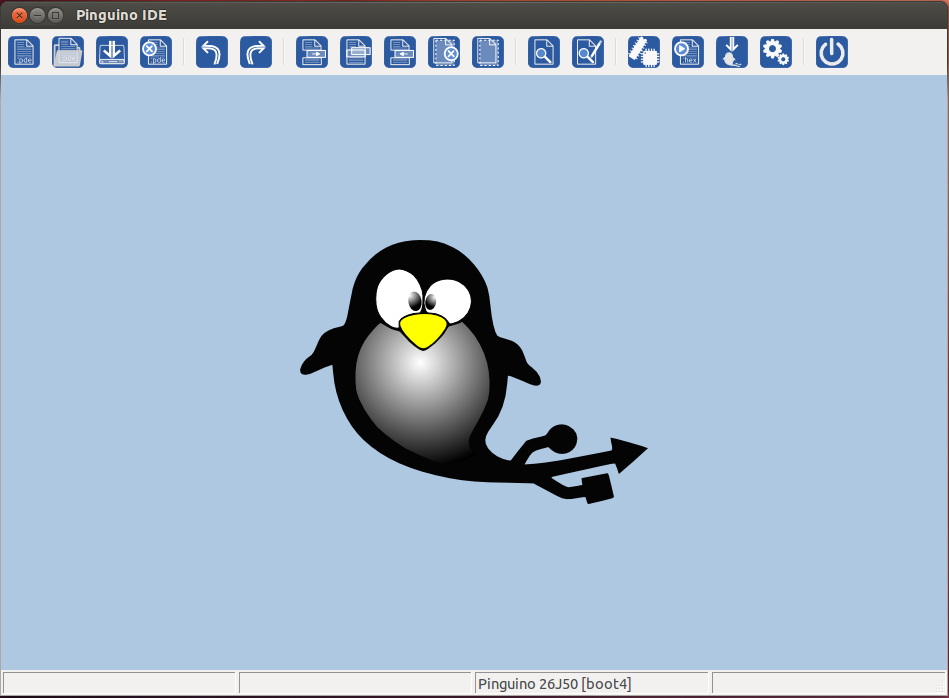
\includegraphics [width=0.9\textwidth]{Pinguino_IDE_inicio.png}
\end{figure}

Lo primero que tenemos que hacer es configurar el hw que estamos
usando. Entramos en el menú correspondiente y, suponiendo que usamos
la placa propuesta, lo configuramos como aparece en la figura
\ref{fig:cfg_micro}

\begin{figure}
  \centering
  \caption{Configuración del micro}
  \label{fig:cfg_micro}
  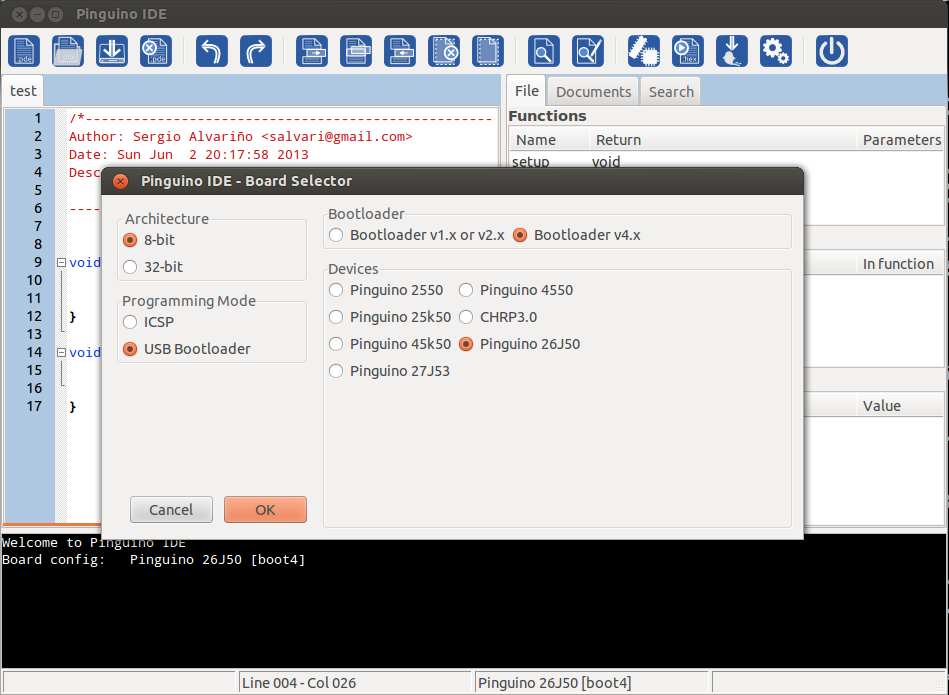
\includegraphics [width=0.9\textwidth]{Pinguino_IDE_cfg_micro.png}
\end{figure}

Una vez configurado el micro, ya estamos listos para compilar y cargar
nuestro primer programa:

\begin{verbatim}
void setup() {
    // run once:
}

void loop() {
    // run repeatedly
    CDC.println("\n\r ¡¡¡Hola Bricolabs!!!")
}
\end{verbatim}

Lo escribimos en la ventana de código (o lo cargamos de la carpeta de
ejemplos) y compilamos con el botón correspondiente del IDE.

Para cargar el programa en el Pingüino tenemos que entrar en el modo
\emph{bootloader}. El Pingüino entra en modo \emph{bootloader} durante
cinco segundos en dos ocasiones:
\begin{itemize}
\item cuando lo encendemos o
\item cuando pulsamos el botón de reset.
\end{itemize}
  
Así que si ya lo tenemos conectado pulsamos el reset, de lo contrario
lo conectamos a un puerto usb de nuestro PC y tenemos cinco segundos
para pulsar el botón de upload de nuestro IDE.

Si todo va bien veremos los mensajes de carga del programa en el
hardware, como en la figura \ref{fig:upload}

\begin{figure}
  \centering
  \caption{Upload}
  \label{fig:upload}
  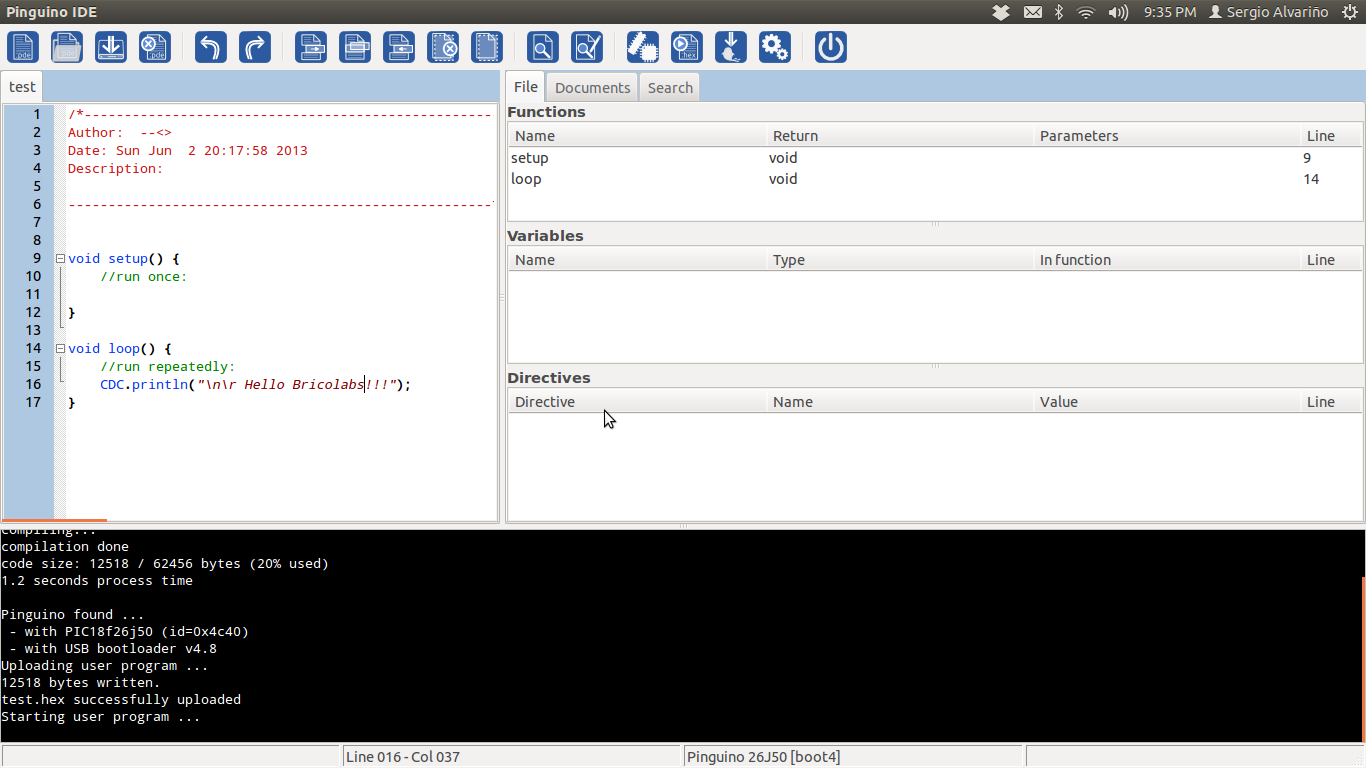
\includegraphics [width=0.9\textwidth]{Upload.png}
\end{figure}

Ya solo falta comprobar que nuestro Pingüino está enviando los
mensajes correspondientes por el puerto USB.

Lo típico es que Ubuntu haya mapeado el dispositivo USB en el puerto
\textbf{ttyACM0}, pero si algo falla o no es ese puerto lo podemos
comprobar ejecutando:
{\tiny
\begin{verbatim}
$ tail /var/log/syslog
Jun  3 02:40:50 madouc kernel: [28973.988017] usb 2-1.4: new full-speed USB device number 51 using ehci_hcd
Jun  3 02:40:50 madouc mtp-probe: checking bus 2, device 51: "/sys/devices/pci0000:00/0000:00:1d.0/usb2/2-1/2-1.4"
Jun  3 02:40:50 madouc mtp-probe: bus: 2, device: 51 was not an MTP device
Jun  3 02:41:00 madouc kernel: [28984.205389] usb 2-1.4: USB disconnect, device number 51
Jun  3 02:41:02 madouc kernel: [28986.449496] usb 2-1.4: new full-speed USB device number 52 using ehci_hcd
Jun  3 02:41:02 madouc kernel: [28986.544948] cdc_acm 2-1.4:1.0: This device cannot do calls on its own. It is not a modem.
Jun  3 02:41:02 madouc kernel: [28986.544996] cdc_acm 2-1.4:1.0: ttyACM0: USB ACM device
Jun  3 02:41:02 madouc mtp-probe: checking bus 2, device 52: "/sys/devices/pci0000:00/0000:00:1d.0/usb2/2-1/2-1.4"
Jun  3 02:41:02 madouc mtp-probe: bus: 2, device: 52 was not an MTP device
\end{verbatim}
}

Una vez que tenemos localizado el puerto hacemos:
\begin{verbatim}
$ cat /dev/ttyACM0
¡¡¡Hola Bricolabs!!!

¡¡¡Hola Bricolabs!!!

¡¡¡Hola Bricolabs!!!
....
\end{verbatim}

\section{Peculiaridades}
\label{sec:peculiar}

Hay dos cosas que me hicieron perder un montón de tiempo a la hora de
probar el Pingüino.

La primera es la configuración de los dispositivos USB; ya os lo he
contado en el proceso de instalación del IDE. El problema es que yo
esperaba que el Pingüino se comportase como el Arduino y Ubuntu lo
mapease a un interfaz ttyACMx, pero no funciona así. Ubuntu solo
``ve'' al Pingüino en modo bootloader y además no lo ``ve'' como un
RS-232 así que no lo mapea a ACM.

Sólo veremos el Pingüino mapeado a un dispositivo ACM, igual que el
Arduino, cuando le carguemos un programa para que el Pingüino
\textbf{haga uso del puerto USB}. Un programa como el que hemos usado
en nuestro ejemplo levantará el puerto USB del Pingüino como
dispositivo USB ACM y Ubuntu lo mapeará a un interfaz ttyACMx.

\section{Consideraciones de cara a un Quick Hacking}
\label{sec:qh_opciones}


Algunas consideraciones de cara a celebrar un Quick Hacking, es decir un taller basado en Pingüino.
\begin{itemize}
\item Yo creo que el Pingüino tiene una ventaja sobre el Shrimp de cara a hacer un taller. Los asistentes se llevarían un paquete completo y funcional ya que el Pingüino incluye el puerto USB.
\item Podríamos comprar solo los PIC 18F26J50 con el bootloader pre-cargado y los componentes sueltos y montarlo en breadboard como el shrimp.
Esta opción simplifica la infraestructura necesaria para impartir el taller puesto que ya no habría que soldar.
\item Hay que añadir el material necesario para hacer algún montaje, por ejemplo si vamos a hacer el típico blink necesitamos led y resistencia, etc. etc.
\item Yo prepararía algo de documentación para los asistentes, aunque solo fuera un pequeño triptico con información clave de la actividad y/o una ``cheat sheet'' del Pingüino.
\end{itemize}


\section{Enlaces interesantes}
\label{sec:enlaces}

\begin{itemize}
\item La página oficial de Pingüino: \url{http://www.pinguino.cc/}
\item La wiki de Pingüino:
  \url{http://wiki.pinguino.cc/index.php/Main_Page}, enlazada también
  desde la página anterior.
\item La página del IDE en GoogleCode: \url{https://code.google.com/p/pinguino32/}
\item Los foros del proyecto: \url{http://forum.pinguino.cc/index.php}
\item Grupo de Google:
  \url{https://groups.google.com/forum/?fromgroups#!forum/pinguinocard}
\item Página de Olimex, un fabricante: \url{https://www.olimex.com/}
\end{itemize}


\end{document}